
\section{Mehrdimensionale Integralrechnung}

\subsection{Lebesgue Maß}

Für offene Intervalle $(a_i,b_i) \subset \mathbb{R}$ mit $a_i \leq b_i$ nennen wir $I := (a_1,b_1) \times \cdots \times (a_n,b_n)$ einen $n$-dimensionalen Quader 
und $\bar{I}:= [a_1, b_1] \times \cdots \times [a_n,b_n]$ seinen Abschluss. Wir definieren das Volumen 
\begin{align*}
\text{vol} (I):=   \prod_{i = 1}^n (b_i -a_i)  \; .
\end{align*}

Mit $\mathbb{I}(n): = \{   (a_1,b_1) \times \cdots \times (a_n,b_n) \; | \;  (a_i, b_i) \subset \mathbb{R} \}$ bezeichnen wir die Menge aller $n$-dimensionalen Quader und mit $\mathbb{I}^0(n): = \{   (a_1,b_1) \times \cdots \times (a_n,b_n) \; | \;  (a_i, b_i) \subset \mathbb{R}  \text { und } a_k = b_k \text{ für ein k}\}$ die Menge der degenerierten Quader.  
Für eine Menge $A \subset \mathbb{R}^n$ bezeichnen wir eine Menge von Quadern $\{ I_j \; | \;  I_j \in \mathbf{I}(n)  \}$ mit $A \subset \bigcup_j I_j$ als Hüllquader für $A$.
\begin{Definition}[Lebesguesche äußere Maß]
Für eine Menge $A \subset \mathbb{R}^n$ definieren wir das Lebesguesche äußere Maß durch 
\begin{align*}
\mu (A):=   \inf \biggl \{ \sum_{j=1}^{\infty}   \text{vol} (I_j)\; ; \; I_j \in \mathbb{I}(n); A \subset \bigcup_{j= 1}^{\infty} I_j \biggr \} 
\end{align*}
Falls für alle Hüllquader $\text{vol} (I_j) = \infty$ gilt, so setzen wir $\mu (A) = \infty$.
\end{Definition}

\begin{Definition}[Erinnerung Infimum]
\end{Definition}

\begin{Definition}[Nullmenge]
Eine Menge $N \subset \mathbb{R}^n$ mit $\mu (N) = 0$ heißt Nullmenge.
\end{Definition}


\begin{Bemerkung}
\label{massmonton}
Für $A \subset B \subset \mathbb{R}^n$ ist $\mu(A) \leq \mu(B)$
\end{Bemerkung}
\begin{proof}
Da $A \subset B$ Teilmenge ist, sind Hüllquader von $B$ sind auch Hüllquader von $A$ und damit  $\mu(A) \leq \mu(B)$.
\end{proof}

\begin{Satz}[$\sigma$-subadditivität]
Sei $A_j \subset \mathbb{R}^n$ eine Folge von Mengen. Dann gilt
\begin{align*}
\mu (\bigcup_j^{\infty} A_j ) \leq \sum_{i=1}^{\infty} \mu(A_j)
\end{align*}
\end{Satz}
\begin{proof}
Für jedes $A_j$ und $\epsilon > 0$ können wir  eine geeignete Überdeckung  $A_j \subset \bigcup_k  K_{j,k}$ mit Hüllquadern $K_{j,k}$ finden, so dass 
 $\sum_k \text{vol} (K_{j,k}) \leq \mu(A_j) + \frac{\epsilon}{2^{j+1}}$.
Da $ \bigcup_j A_j \subset \bigcup_j \bigcup_k  K_{j,k}$ eine Überdeckung mit Hüllquadern ist, folgt
\begin{align*}
\mu \biggl (  \bigcup A_j  \biggr) \leq \sum_j \sum_k \text{vol} (K_{j,k}) \leq  \bigl( \sum_j  \mu(A_j) + \frac{\epsilon}{2^{j+1}} \bigr)  = \bigl (\sum_j \mu(A_j) \bigr ) + \epsilon
\end{align*}
(Die letzte Gleichung beruht auf dem Wert der \href{https://de.wikipedia.org/wiki/Geometrische_Reihe}{geometrischen Reihe}).
Da die letzte Aussage für beliebiges $\epsilon > 0$ gilt, folgt die Behauptung.
\end{proof}


\begin{Bemerkung}
\label{volimu}
Für $I \in \mathbb{I}(n)$ gilt $\mu(I) = \text{vol}(I)$.
\end{Bemerkung}
\begin{proof}
Seien  $I_j \in \mathbb{I}(n)$ mit $I \subset \bigcup_j  I_j$. Da $I$ beschränkt und abgeschlossen ist, ist $I$ kompakt. Damit reichen endlich 
viele Intervalle, um $I  \subset  \bigcup_{j=1}^n  I_j$ zu überdecken. Für endlich viele Intervalle ist es einfach zu zeigen, dass
$$\text{vol} (I) \leq \sum_{j=1}^n \text{vol} (I_j) $$
gilt. Damit folgt die Behauptung.
\end{proof}

\begin{Satz}
Für $I \in \mathbb{I}(n)$  und $A \subset \mathbb{R}^n$ mit $I \subset A \subset \bar{I}$ gilt $\mu (A) = \text{vol}(I)$.
\end{Satz}
\begin{proof}
Mit $I_0:=  I$ und $I_j := \emptyset$ ist $I \subset \bigcup_j I_j$ und damit gilt 
\begin{align*}
\mu(I) \leq \sum_j \text{vol}(I_j) = \text{vol}(I)
\end{align*}

Es sei $\mathcal{A}_0 := \{ A  \in \mathbb{R}^n  \; | \;  I^0 \subset A \subset \bar{I^0}  \text{  mit } I^0 \in \mathbb{I}^0(n) \}$. Für $A_0 \in \mathcal{A}_0$ gibt es 
$\epsilon > 0$ und $I_{\epsilon} \in \mathbb{I}(n)$ mit $A \subset I_{\epsilon}$ und $\text{vol} (I_{\epsilon})  \leq epsilon$ und damit $\mu(A_0) = 0$.
Zu $I \in \mathbb{I}(n)$ gibt es $2n$-Seiten $J_j \in \mathcal{A}_0$ mit 
$\bar{I} = I \cup \bigcup{j= 1}^{2n} J_j$. Aus der $\sigma$-subadditivität folgt
\begin{align*}
\mu(\bar{I})  \leq \mu(I) + \sum_{j=1}^{2n} \mu(J_j) = \mu (I)
\end{align*}
 Für $I \subset A \subset \bar{I}$ folgt damit und mit der Monotonie
$$ \mu(I) = \mu(A) = \mu(\bar{I}) \;. $$
Mit Bemerkung \ref{volimu} folgt die Behauptung.

\end{proof}


Es sei $A, D \subset \mathbb{R}^n$  beschränkte Teilmenge mit $A \subset D$.  
Man kann einerseits das Volumen $\mu(A)$, als auch das Volumen 
$\mu_D(A) :=  \mu(D) - \mu(D  \setminus  A)$ berechnen. Man approximiert hierbei das Volumen von $A$ einmal mit Hüllquadern von außen und einmal von innen.
 
\begin{figure}[!tbp]
  \centering
  \begin{minipage}[b]{0.49\textwidth}
    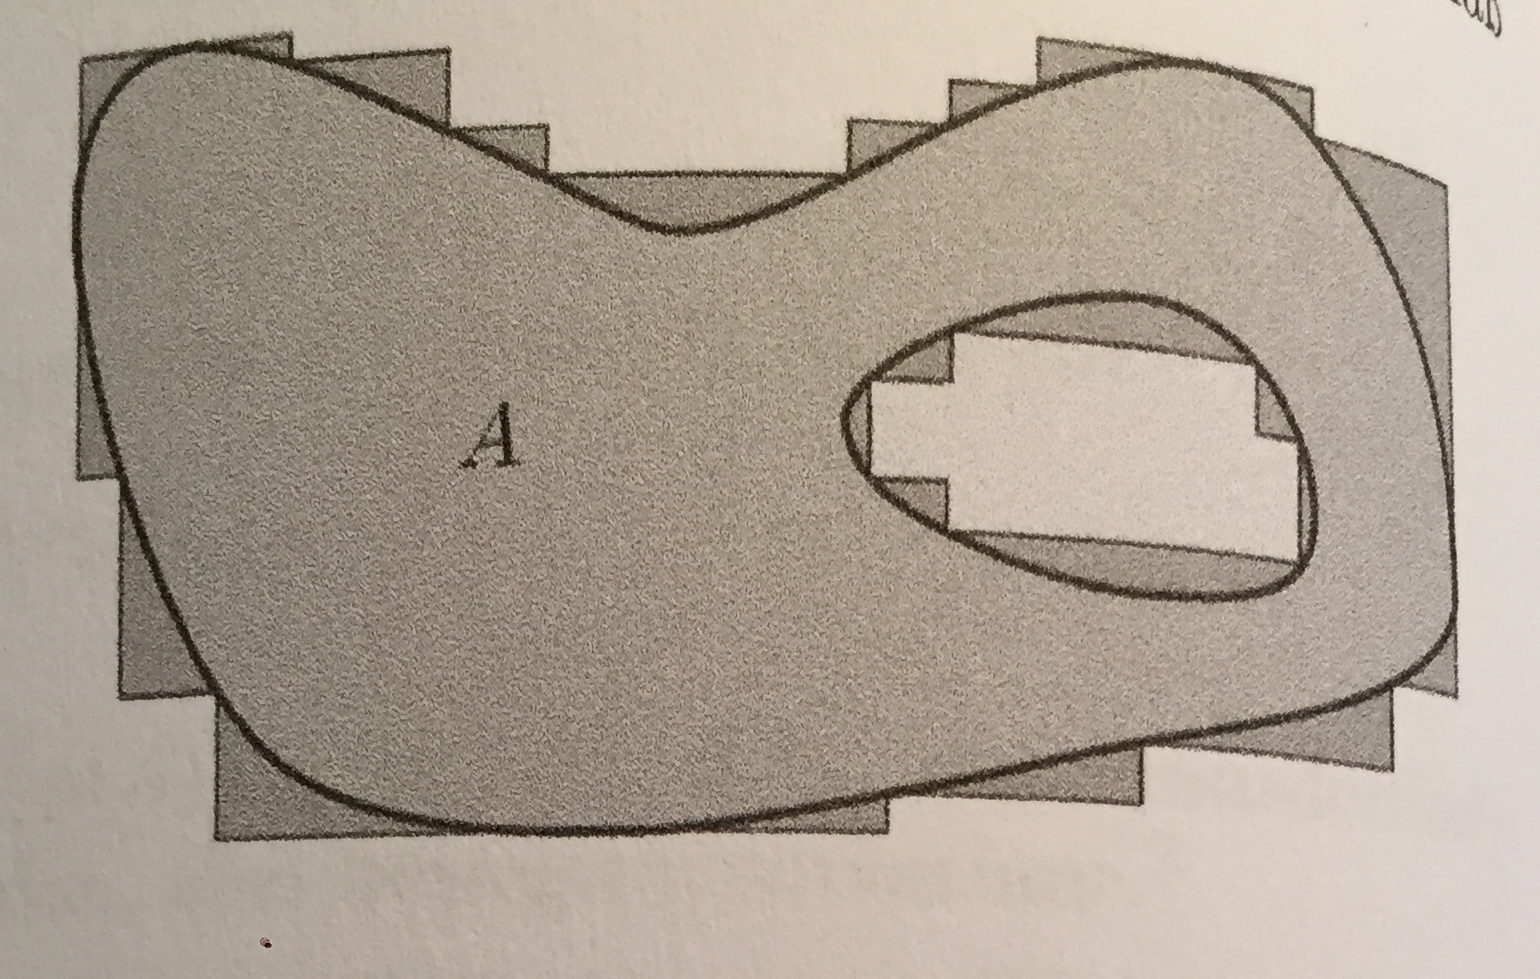
\includegraphics[width=1.0\textwidth]{images/am}
    \caption{Äußeres Maß}
  \end{minipage}
  \hfill
  \begin{minipage}[b]{0.49\textwidth}
    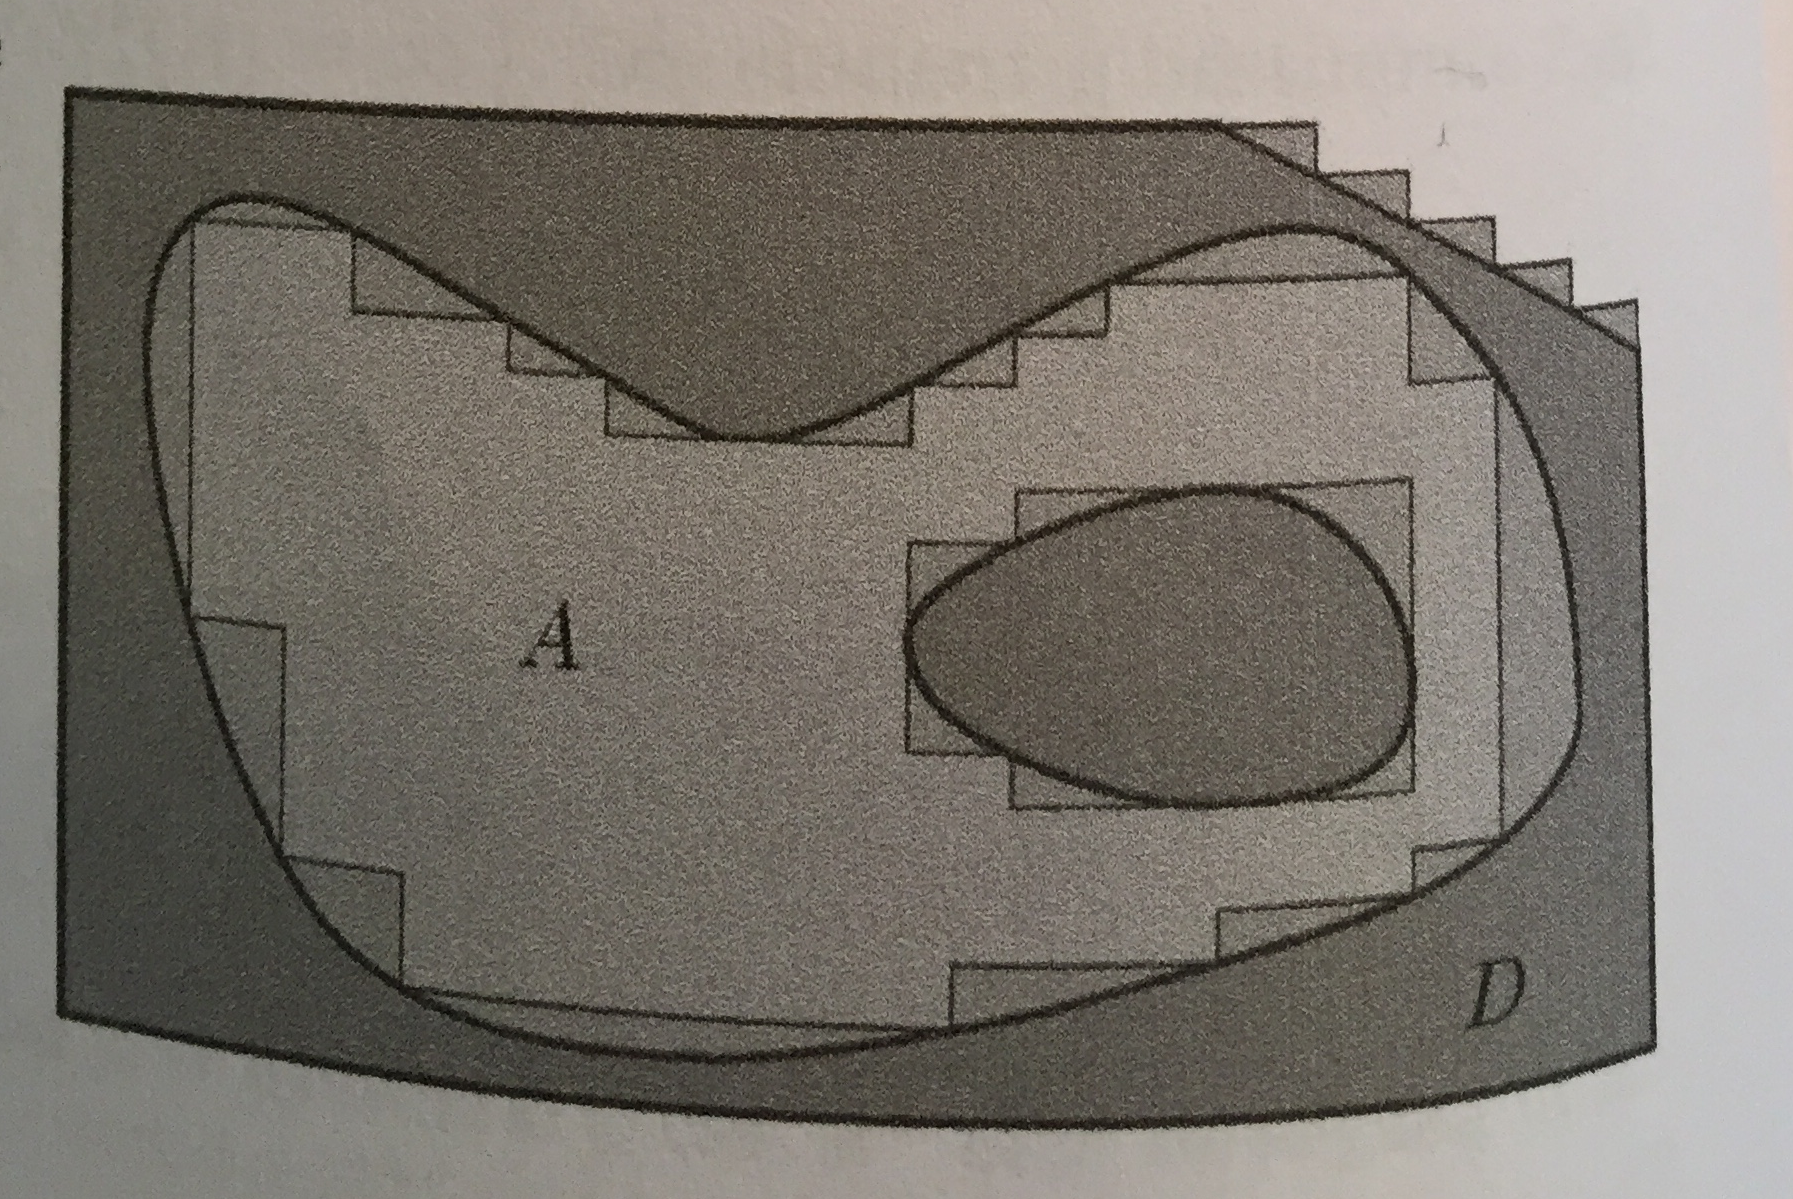
\includegraphics[width=1.0\textwidth]{images/im}
    \caption{Inneres Maß}
  \end{minipage}
\end{figure}

Es ist daher sinnvoll von einer messbaren Menge zu sprechen, wenn diese beiden Volumen übereinstimmen, also
$\mu_D(A) = \mu(A)$ gilt. Dies ist gleichbedeutend mit der Bedingung $\mu(D) = \mu(A) + \mu(D  \setminus A)$. 
Für festes $D$ wären somit alle Mengen $A$ messbar, für die das äußere Lebesgue Maß additiv ist auf der Zerlegung $D = A \cup D \setminus A$. 
Lässt man die Bedingungen der Beschränktheit und $A \subset D$ fallen, gelangt man zu folgender Definition.

\begin{Definition}[$\mu$-messbare Menge]
Eine Menge $A \subset \mathbb{R}^n$ heißt messbar, falls für alle $D \subset  \mathbb{R}^n$ gilt
\begin{align*}
\mu(D) =  \mu(A \cap D) + \mu(A^c \cap D)
\end{align*}
Da wir die $\sigma$-subadditivität bereits nachgewiesen haben, können wir diese Bedingung auf
\begin{align*}
\mu(D) \geq  \mu(A \cap D) + \mu(A^c \cap D)
\end{align*}
reduzieren. Die Menge aller messbaren Mengen bezeichnen wir mit $\mathcal{A}$.
\end{Definition}

\begin{Bemerkung}
Nullmengen sind messbar.
\end{Bemerkung}
\begin{proof}
Es sei $N, D \subset \mathbb{R}^n$ mit $\mu(N)= 0$. Wegen der Monotonie von $\mu$ ist $0 \leq \mu (N \cap D) \leq \mu(N) = 0$ und somit ist $N \cap D$ auch eine Nullmenge. Wir erhalten damit und nochmaliger Monotonie von $\mu$
$$ \mu(N \cap D) + \mu (N^c \cap D) =  \mu (N^c \cap D) \leq \mu(D) $$
und damit ist $N$ messbar.
\end{proof}



\subsubsection*{$\sigma$-Algebra der messbaren Mengen}
Die Menge der messbaren Mengen $\mathcal{A}$ hat einige besondere Eigenschaften. Wir geben hier nur diese Eigenschaften ohne Beweis an. Die Beweise verwenden im wesentlichen Techniken, die wir bereits kennengelernt haben.
\begin{itemize}
\item Für eine Folge $A_i \in \mathcal{A}$ von messbaren Mengen mit $A_i \cap A_j  =  \emptyset$ ist $\mu (\bigcup_i A_i ) = \sum_i \mu(A_i)$.
\item Ist $A \in \mathcal{A} $, so ist auch $A^c \in \mathcal{A} $.
\item Für eine Folge $A_i \in \mathcal{A}$ messbarer Mengen  ist $\bigcup_i A_i \in \mathcal{A}$ messbar.
\end{itemize}



\begin{Satz}[Charakterisierung messbarer Mengen]
Eine Menge $A$ ist genau dann messbar, wenn $A = S \cup N$, wobei $N$ eine Nullmenge und $S$ Vereinigung von kompakten Mengen ist.
\end{Satz}


\subsection{Lebesgue Integral}
 Eine Treppenfunktion ist eine Funktion, die auf endlich vielen Quadern einen konstanten Wert hat und sonst null ist. 

\begin{Definition}
Für eine Teilmenge $A \subset \mathbb{R}^n$ heißt
$$ 1_A (x): = \begin{cases} 1 \text{  falls }   x \in A  \\  0  \text{  sonst}  \end{cases}$$
heißt Indikatorfunktion.
\end{Definition}

\begin{Definition}
Eine Funktion 
$$ \varphi(x) := \sum_{k=1}^m c_k 1_{I_k}$$ mit $c_k \in \mathbb{R}$ und $I_k \in \mathbb{I}(n)$ mit $I_l \cap I_h = \emptyset$ für $i \neq j$
heißt Treppenfunktion.
\end{Definition}

\begin{Bemerkung}
Seien $\varphi(x) =   \sum_{k=1}^m  c_k 1_{I_k}$ und $\psi(x) =  \sum_{j=1}^l  u_j 1_{I_j}$. Dann definiert
$(\varphi + \psi)(x) := \sum_{k=1}^m \sum_{j=1}^l   (c_k + u_j) 1_{I_{k,j}}$ mit $I_{k,j}:= I_k \cap I_j$ eine Treppenfunktion (nach entsprechender Umnummerierung zu einem einzigen Summenzeichen).
\end{Bemerkung}


\begin{Definition}
Für eine Treppenfunktion $ \varphi(x) := \sum_{k=1}^m c_k 1_{I_k}$ definieren wir das Integral durch
$$\int_{\mathbb{R}^n} \varphi d\mu := \sum_{k =1}^m  c_k \mu(I_k) \; . $$
\end{Definition}

\begin{Satz}
Seien $\varphi(x) =   \sum_{k=1}^m  c_k 1_{I_k}$ und $\psi(x) =  \sum_{j=1}^l  u_j 1_{I_j}$ zwei Treppenfunktionen.
Für das Integral von Treppenfunktion gilt:
\begin{itemize}
\item Ist $\varphi(x) = \psi(x)$ für alle $x$, dann ist $\int_{\mathbb{R}^n} \varphi d\mu = \int_{\mathbb{R}^n} \psi d\mu$ (Das integral hängt nicht von der Zerlegung der Treppenfunktion ab und  ist wohldefiniert)
\item $\int_{\mathbb{R}^n} \alpha \varphi  + \beta \psi d\mu = \alpha \int_{\mathbb{R}^n}  \varphi d\mu + \beta  \int_{\mathbb{R}^n}  \psi d\mu$
\item $ \biggl|  \int_{\mathbb{R}^n} \varphi d\mu  \biggr| \leq \int_{\mathbb{R}^n} | \varphi | d\mu$
\item Ist $\varphi(x) \leq \psi(x)$ für alle $x$, so ist $\int_{\mathbb{R}^n} \varphi d\mu \leq \int_{\mathbb{R}^n} \psi d\mu$ 
\end{itemize}
\end{Satz}

\begin{proof}
Der Beweis wird über eine Vollständige Induktion geführt. Der Induktionsanfang ist einfach zu zeigen. 
Wir nehmen an, die Aussage gilt für alle Dimensionen $k < n$.
Zerlege $\mathbb{R}^n = \mathbb{R}^p \times \mathbb{R}^{n-p}$. Jeder Quader $I \in \mathbb{I}(n)$ zerlegt sich damit ebenfalls in ein Produkt 
$I = I' \times I''$ mit $I'  \in \mathbb{I}(p)$ und  $I''  \in \mathbb{I}(n-p)$ und für $z = (x,y) \in  \mathbb{R}^p \times \mathbb{R}^{n-p}$ gilt $1_{I} (z) = 1_{I'}(x) \cdot 1_{I''}(y)$. Es sei nun $\varphi(z):=   \sum_{k=1}^m  c_k 1_{I_k}(z)$ eine Treppenfunktion auf $ \mathbb{R}^p \times \mathbb{R}^{n-p}$. Für jedes $y \in \mathbb{R}^{n-p}$ definiert  $\varphi_y(x)=   \sum_{k=1}^m  c_k 1_{I''_k}(y) \cdot 1_{I'_k}(x)$ eine Treppenfunktion auf $\mathbb{R}^{n-p}$. 
Nach Induktionsvoraussetzung hängt das Integral 
$$\int_{\mathbb{R}^p}  \varphi_y(x) d \mu' = \sum_{k=1}^m  c_k \mu'(I'_k)  \cdot 1_{I''_k}(y)  =: \phi(y)$$
nicht von der Zerlegung der Treppenfunktion ab. $\phi(y)$ ist wiederum eine Treppenfunktion auf $\mathbb{R}^{n-p}$ und Nach Induktionsvoraussetzung hängt das Integral 
$$\int_{\mathbb{R}^{n-p}}  \phi(y) d \mu'' = \sum_{k=1}^m  c_k \mu'(I'_k)  \cdot \mu'' (I''_k)(y) $$
nicht von der Zerlegung der Treppenfunktion ab. Somit gilt
$$\int_{\mathbb{R}^{n-p}} \int_{\mathbb{R}^p}  \varphi_y(x) d \mu'  d \mu''  =   \sum_{k=1}^m  c_k \mu'(I'_k)  \cdot \mu''(I''_k)(y) = \sum_{k=1}^m  c_k  \mu(I_k)  = \int_{\mathbb{R}^n} \varphi(z) d\mu\;.$$
Die linke Seite hängt  damit nicht von der Zerlegung der Treppenfunktion ab und alle Behauptungen können so auf den Fall $n=1$ zurückgeführt werden.
\end{proof}

\begin{Bemerkung}[Satz von Fubini für Treppenfunktionen]
Es gilt $$\int_{\mathbb{R}^n} \varphi(x,y) d \mu = \int_{\mathbb{R}^{n-p}} \biggl (\int_{\mathbb{R}^{p}}  \varphi(x,y) d \mu' \biggr ) d \mu''$$
\end{Bemerkung}
\begin{proof}
Siehe Beweis des letzten Satzes.
\end{proof}


